\subsection{Radix Sort}

\subsubsection{Ý tưởng}

Radix Sort sắp xếp các phần tử bằng cách xử lý từng chữ số của các số từ hàng thấp nhất (hàng đơn vị) đến hàng cao nhất. Thuật toán này sử dụng Counting Sort như một bước phụ trợ để sắp xếp theo từng chữ số. \cite[p.~106--107]{hoang2008}

\subsubsection{Mã giả}

\begin{algorithm}[H]
\caption{Radix Sort \cite[p.~256]{weiss2013} \cite{code-radix}}
\label{radix-sort}

\SetKwFunction{CountingSortByDigit}{CountingSortByDigit}
\SetKwFunction{RadixSort}{RadixSort}
\SetKwProg{Fn}{Function}{:}{}
\Fn{\CountingSortByDigit {arr\KwSty{[ ]}, n, exp}}{
    $count[10] \gets \{0\}$ \tcp{Mảng đếm cho 10 chữ số}
    $output[n] \gets \{0\}$ \tcp{Mảng kết quả}
    \For{$i \gets 0$ \KwTo $n-1$}{
        $index = (arr[i] \hspace{0.2cm} / \hspace{0.2cm} exp) \% 10$ \\
        $count[index]++$
    }
    \For{$i \gets 1$ \KwTo $9$}{
        $count[i] += count[i-1]$
    }
    \For{$i \gets n-1$ \KwSty{downto} $0$}{
        $index = (arr[i] \hspace{0.2cm} / \hspace{0.2cm} exp) \% 10$ \\
        $output[count[index] - 1] = arr[i]$ \\
        $count[index]--$
    }
    \For{$i \gets 0$ \KwTo $n-1$}{
        $arr[i] = output[i]$
    }
}
\textbf{end function}

\Fn{\RadixSort {arr\KwSty{[ ]}, n}}{
    $maxVal \gets max(a,n)$ \tcp{Tìm giá trị lớn nhất để biết số chữ số}
    $exp \gets 1$ \\
    \While{$maxVal / exp > 0$}{
        \CountingSortByDigit{arr, n, exp} \\
        $exp \, *= \, 10$
    }
}
\textbf{end function}
\end{algorithm}

\subsubsection{Ví dụ}

Giả sử ta có mảng ban đầu với $n=7$ như sau:
\begin{center}
    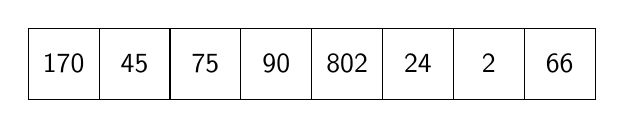
\begin{tikzpicture}[node distance=0cm, scale=0.9, font=\sffamily, every node/.style={minimum width=0.9cm, minimum height=0.9cm, outer sep=0pt, anchor = west}, line join=miter, line cap=rect]
        \node[draw, fill=white] at (9, 0) {170};
        \node[draw, fill=white] at (10, 0) {45};
        \node[draw, fill=white] at (11, 0) {75};
        \node[draw, fill=white] at (12, 0) {90};
        \node[draw, fill=white] at (13, 0) {802};
        \node[draw, fill=white] at (14, 0) {24};
        \node[draw, fill=white] at (15, 0) {2};
        \node[draw, fill=white] at (16, 0) {66};
    \end{tikzpicture}
\end{center}

\textbf{Bước 1:} Sắp xếp theo chữ số hàng đơn vị $(exp = 1)$.

\begin{center}
    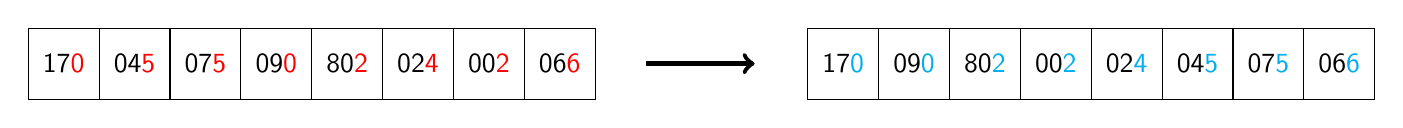
\begin{tikzpicture}[node distance=0cm, scale=0.9, font=\sffamily, every node/.style={minimum width=0.9cm, minimum height=0.9cm, outer sep=0pt, anchor = west}, line join=miter, line cap=rect]
        \node[draw, fill=white] at (0, 0) {17\textcolor{red}{0}};
        \node[draw, fill=white] at (1, 0) {04\textcolor{red}{5}};
        \node[draw, fill=white] at (2, 0) {07\textcolor{red}{5}};
        \node[draw, fill=white] at (3, 0) {09\textcolor{red}{0}};
        \node[draw, fill=white] at (4, 0) {80\textcolor{red}{2}};
        \node[draw, fill=white] at (5, 0) {02\textcolor{red}{4}};
        \node[draw, fill=white] at (6, 0) {00\textcolor{red}{2}};
        \node[draw, fill=white] at (7, 0) {06\textcolor{red}{6}};
        
        \draw[->, line width=0.6mm] (8.75, 0) -- (10.25, 0);
        
        \node[draw, fill=white] at (11, 0) {17\textcolor{cyan}{0}};
        \node[draw, fill=white] at (12, 0) {09\textcolor{cyan}{0}};
        \node[draw, fill=white] at (13, 0) {80\textcolor{cyan}{2}};
        \node[draw, fill=white] at (14, 0) {00\textcolor{cyan}{2}};
        \node[draw, fill=white] at (15, 0) {02\textcolor{cyan}{4}};
        \node[draw, fill=white] at (16, 0) {04\textcolor{cyan}{5}};
        \node[draw, fill=white] at (17, 0) {07\textcolor{cyan}{5}};
        \node[draw, fill=white] at (18, 0) {06\textcolor{cyan}{6}};
    \end{tikzpicture}
\end{center}

\textbf{Bước 2:} Sắp xếp theo chữ số hàng hàng chục $(exp = 10)$.

\begin{center}
    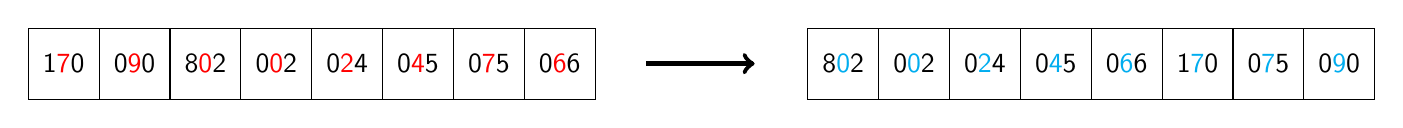
\begin{tikzpicture}[node distance=0cm, scale=0.9, font=\sffamily, every node/.style={minimum width=0.9cm, minimum height=0.9cm, outer sep=0pt, anchor = west}, line join=miter, line cap=rect]
        \node[draw, fill=white] at (0, 0) {1\textcolor{red}{7}0};
        \node[draw, fill=white] at (1, 0) {0\textcolor{red}{9}0};
        \node[draw, fill=white] at (2, 0) {8\textcolor{red}{0}2};
        \node[draw, fill=white] at (3, 0) {0\textcolor{red}{0}2};
        \node[draw, fill=white] at (4, 0) {0\textcolor{red}{2}4};
        \node[draw, fill=white] at (5, 0) {0\textcolor{red}{4}5};
        \node[draw, fill=white] at (6, 0) {0\textcolor{red}{7}5};
        \node[draw, fill=white] at (7, 0) {0\textcolor{red}{6}6};
        
        \draw[->, line width=0.6mm] (8.75, 0) -- (10.25, 0);
        
        \node[draw, fill=white] at (11, 0) {8\textcolor{cyan}{0}2};
        \node[draw, fill=white] at (12, 0) {0\textcolor{cyan}{0}2};
        \node[draw, fill=white] at (13, 0) {0\textcolor{cyan}{2}4};
        \node[draw, fill=white] at (14, 0) {0\textcolor{cyan}{4}5};
        \node[draw, fill=white] at (15, 0) {0\textcolor{cyan}{6}6};
        \node[draw, fill=white] at (16, 0) {1\textcolor{cyan}{7}0};
        \node[draw, fill=white] at (17, 0) {0\textcolor{cyan}{7}5};
        \node[draw, fill=white] at (18, 0) {0\textcolor{cyan}{9}0};
    \end{tikzpicture}
\end{center}

\textbf{Bước 3:} Sắp xếp theo chữ số hàng hàng trăm $(exp = 100)$.

\begin{center}
    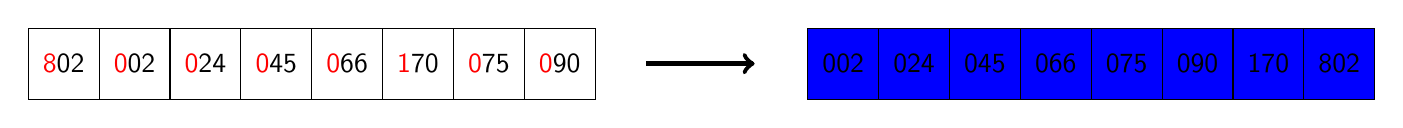
\begin{tikzpicture}[node distance=0cm, scale=0.9, font=\sffamily, every node/.style={minimum width=0.9cm, minimum height=0.9cm, outer sep=0pt, anchor = west}, line join=miter, line cap=rect]
        \node[draw, fill=white] at (0, 0) {\textcolor{red}{8}02};
        \node[draw, fill=white] at (1, 0) {\textcolor{red}{0}02};
        \node[draw, fill=white] at (2, 0) {\textcolor{red}{0}24};
        \node[draw, fill=white] at (3, 0) {\textcolor{red}{0}45};
        \node[draw, fill=white] at (4, 0) {\textcolor{red}{0}66};
        \node[draw, fill=white] at (5, 0) {\textcolor{red}{1}70};
        \node[draw, fill=white] at (6, 0) {\textcolor{red}{0}75};
        \node[draw, fill=white] at (7, 0) {\textcolor{red}{0}90};
        
        \draw[->, line width=0.6mm] (8.75, 0) -- (10.25, 0);
        
        \node[draw, fill=blue] at (11, 0) {002};
        \node[draw, fill=blue] at (12, 0) {024};
        \node[draw, fill=blue] at (13, 0) {045};
        \node[draw, fill=blue] at (14, 0) {066};
        \node[draw, fill=blue] at (15, 0) {075};
        \node[draw, fill=blue] at (16, 0) {090};
        \node[draw, fill=blue] at (17, 0) {170};
        \node[draw, fill=blue] at (18, 0) {802};
    \end{tikzpicture}
\end{center}

\subsubsection{Độ phức tạp thuật toán}

\begin{itemize}
    \item Độ phức tạp thời gian \cite[p.~213]{cormen2022}
    \begin{itemize}[label=$\circ$]
        \item Trường hợp tốt nhất: $O\left(d\times\left(n+k\right)\right)$. 
        Khi $n$ lớn và $k$ nhỏ. 
        \item Trường hợp xấu nhất: $O\left(d\times\left(n+k\right)\right)$. 
        Trường hợp xấu nhất xảy ra khi giá trị lớn nhất trong mảng có nhiều 
        chữ số $(d)$ lớn và phạm vi giá trị của mỗi chữ số $(k)$ lớn. Tuy nhiên, 
        hiệu suất vẫn được đảm bảo bởi tính ổn định của Counting Sort.
        \item Trường hợp trung bình: $O\left(d\times\left(n+k\right)\right)$. 
        Trường hợp này xảy ra khi các giá trị trong mảng được phân bố ngẫu nhiên. 
        Radix Sort vẫn thực hiện d lần Counting Sort với hiệu suất ổn định.
    \end{itemize}
    
    \item Độ phức tạp không gian: $O\left(n+k\right)$. Vì Radix Sort 
    sử dụng không gian phụ từ Counting Sort.

\end{itemize}

Trong đó:

\begin{itemize}[label=$\circ$]
    \item d: Số lượng chữ số của giá trị lớn nhất có trong mảng.
    \item k: Phạm vi giá trị của mỗi chữ số, phụ thuộc vào hệ cơ số 
    mà Radix Sort sử dụng (ví dụ: với hệ thập phân, $k=10$).
\end{itemize}